\documentclass[a5paper]{article}
\usepackage[a5paper, top=17mm, bottom=17mm, left=17mm, right=17mm]{geometry}
\usepackage[utf8]{inputenc}
\usepackage[T2A,T1]{fontenc}
\usepackage[colorlinks,filecolor=blue,citecolor=green,unicode,pdftex]{hyperref}
\usepackage{cmap}
\usepackage[english,russian]{babel}
\usepackage{amsmath}
\usepackage{amssymb,amsfonts,textcomp}
\usepackage{color}
\usepackage{array}
\usepackage{hhline}
\hypersetup{colorlinks=true, linkcolor=blue, citecolor=blue, filecolor=blue, urlcolor=blue, pdftitle=1, pdfauthor=, pdfsubject=, pdfkeywords=}
\usepackage[pdftex]{graphicx}
\usepackage{graphicx}
%\usepackage{literat}
\usepackage{indentfirst}
\usepackage{multirow}
\usepackage{subfig}
\usepackage{tabularx}

\sloppy
\pagestyle{plain}

\title{Подходы к заданию семантики интерпретации диаграмм, основанные на технологии преобразования графов}

\author{В.А.Поляков \and Т.А.Брыксин}
\date{}
\begin{document}

\maketitle
\thispagestyle{empty}

\begin{quote}
\small\noindent
В статье рассматривается задача интерпретации визуальных языков моделирования. Приводится обзор основных основанных на технологии преобразования графов способов описания исполнимой семантики визуальных языков, необходимой для осуществления такой интерпретации. Кратко описывается Dynamic Meta Modeling, анализируются подходы, использующиеся в средстве AToM$^3$ и при организации анимированной интерпретации диаграмм с помощью средства GenGED. В конце статьи приведено сравнение основных подходов к заданию исполнимой семантики, а также делаются выводы относительно применимости рассмотренных подходов при разработке DSM-платформ.
\end{quote}

\section*{Введение}

Существует ряд различных подходов к разработке программного обеспечения. Одним из них является модельно-ориентированна разработка (Model-driven engineering, MDE), в рамках которой разрабатываемая система описывается с разных точек зрения при помощи моделей. Чаще всего для этого используют графические языки. Одним из самых популярных направлений в рамках MDE в настоящее время является предметно-ориентированное моделирование (Domain-specific modeling, DSM)~\cite{koznov1, koznov2, dsmbook}. Суть DSM в активном создании и использовании специализированных языков (Domain-specific languages, DSL) для решения возникающих задач. Такой подход может довольно сильно повысить продуктивность разработчиков за счет сужения предметной области языка и, как следствие, повышения его наглядности и возможности автоматической кодогенерации из него, однако при этом требует создания довольно большого числа инструментов для поддержки DSL --- визуальных редакторов, генераторов кода, документации, тестов и пр., репозиториев моделей, средств осуществляения преобразования моделей и многого другого. Для автоматизации эффективного создания таких DSM-решений для выбранной конкретной области разрабатываются программные окружения, называемые metaCASE-системами или DSM-платформами~\cite{dsm1, dsm4}. 

Для поведенческих визуальных DSL имеет смысл говорить об инструментах, позволяющих осуществлять исполнение и, как следствие, отладку моделей, созданных с помощью таких языков. С помощью таких инструментов разработчик сможет искать ошибки в своих моделях ещё до завершения их создания, а также лучше разобраться в принципах работы разрабатываемой системы, что, в результате, повысит её качество. Ручное создание отладчиков и интерпретаторов для каждого нового предметного языка является очень дорогой и неэффективной работой, поэтому есть необходимость добавить средства автоматизированного создания отладчиков и интерпретаторов создаваемых поведенческих языков в DSM-платформы. Это позволит пользователям таких платформ разрабатывать интерпретаторы и отладчики своих языков вместе с самими языками централизованно и автоматизированно.

Для того, чтобы модель на визуальном языке можно было исполнять, необходимо задать формальную семантику для элементов и конструкций этого языка. Существует множество различных подходов к заданию такой семантики. Основные из них (механизм двухуровневой отладки~\cite{kartashev}, xUML~\cite{xuml}, DMM~\cite{dmm1}, подход, использующийся в средстве EProvide~\cite{eprov1, eprov2}) были разобраны в статье~\cite{part1}. На основе анализа рассмотренных подходов был сделан вывод, что подходы, основанные на технологии преобразования графов, являются наиболее перспективными, т.к. они являются формальными, наглядными и довольно удобными в использовании. Цель данной статьи --- дать подробное описание некоторых основных способов определения и задания семантики исполнения, основанных на преобразованиях графов. 


\section{Семантика языков}

В первом приближении любой язык, текстовый или графический, состоит из двух частей: набора знаков и набора правил, в соответствии с которыми можно объединять знаки в группы, образующие осмысленные конструкции. С более формальной точки зрения в языке выделяют синтаксис, семантику и прагматику. Первое отвечает за составление текста из знаков, второе --- за придание тексту смысла, т.е. за его проекцию в реальные ситуации из предметной области языка или в любую другую формально заданную область, третье --- за то, как данный язык может быть использован пользователем. Семантика позволяет придавать смысл конструкциям, создаваемым с помощью элементов языка, т.е. определяет соответствие их реальным ситуациям из предметной или из любой другой формально определённой области, называемой семантической областью. Семантика интерпретации обеспечивает возможность исполнения конструкций на данном языке как программы.

Разделяют четыре основных вида семантик для языков программирования: операционные, денотационные, аксиоматические и трансляционные. Операционные семантики~\cite{sem2, sem3} являются набором правил, при помощи которых интерпретация программы на данном языке очевидно раскладывается в набор вычислительных шагов. Денотационные семантики~\cite{sem3} обеспечивают проекцию в семантическую область (часто это математические объекты или функции) рекурсивно, т.е. семантика выражений получается из семантики подвыражений. Аксиоматические семантики~\cite{sem1} определяются возможностью вывода из заданного начального набора логических аксиом. Трансляционные семантики~\cite{sem4} состоят из набора правил, последовательное применение которых к модели на исходном языке обеспечивает её преобразование к модели/коду на другом языке, которые уже можно исполнять.

Более подробно с описанием основных типов семантик можно ознакомиться в статье~\cite{part1}. В данной работе будут рассмотрены основные подходы, для которых семантической областью являются графы и их преобразования. Они включают в себя черты как денотационных, так и операционных семантик.

\section{Dynamic Meta Modeling}

Наиболее мощным и, на наш взгляд, хорошо проработанным способом задания семантики визуальных языков, использующим в качестве своей основы технологию преобразования графов, является Dynamic Meta Modeling (далее DMM). Его предложил Ян Хаусман (Jan Hausmann) из университета в Падерборне (Германия) в своей кандидатской диссертации~\cite{dmm1}. DMM можно применить к произвольному визуальному языку несмотря на то, что изложенное в диссертации исследование опирается на UML~\cite{uml}. DMM обладает высокой степенью формальности, ясен и адекватен при определении семантики исполнения визуальных языков и основывается на концепции семантики действий (action semantics), сочетающей в себе черты как денотационной, так и операционной семантики. Подробный обзор и анализ DMM-подхода был произведён в статье~\cite{part1}, здесь же будут описаны лишь его основные черты.

Основной идеей в DMM является тот факт, что модель, созданная при помощи визуального языка, рассматривается как типизированный мультиграф с атрибутами и метками на узлах и рёбрах, допускающий наследование, связанное с возможностью расширения типов узлов и рёбер. Сам же процесс исполнения связан с преобразованиями таких типизированных графов. Задаётся соответствующий набор правил преобразования графов, которые впоследствии поочерёдно применяются к модели.

В общем случае~\cite{graph}, правило преобразования графов состоит из правой и левой части. При применении правила к модели происходит следующее: в модели ищется подграф, совпадающий с левой частью, и заменяется на то, что стоит в правой. При такой замене могут удаляться и добавляться элементы, переставляться концы связей и т.п.

Также в эти правила могу быть добавлены некоторые расширения. Например, отрицающие применение условия (Negative Application Conditions, NAC), универсальное замыкание (Universal Quantification, UQ) и возможность внутри одних правил вызывать для конкретных элементов другие (invocations). Подробнее о них в статье~\cite{part1}.

Среди главных недостатков DMM можно выделить следующие. Несмотря на его универсальность, понятность и наглядность как при задании семантики, так и при самой интерпретации, он не был реализован. Заметим, что задача поиска пографа в графе является NP-полной, поэтому данный подход в общем случае имеет высокую алгоритмическую сложность.

\section{AToM$^3$}

Среди открытых DSM-платформ, позволяющих создавать новые DSL и соответствующие им DSM-пакеты, помимо среды моделирования Eclipse Modeling Project~\cite{koznov3} существует также ряд других (см., например,~\cite{dsm2, dsm3, dsm4}). Среди них можно выделить кроссплатформенный  проект AToM$^3$ (A Tool for Multi-Formalism and Meta-Modelling,~\cite{atom2}), написанный целиком на языке Python. Кроме традиционного для  таких платформ  функционала AToM$^3$ предоставляет возможность трансляции моделей, записанных как на одном визуальном языке, так и на разных, оптимизации (по сути, замене конструкций более эффективными) и симуляции (интерпретации) моделей, а также генерации кода по моделям. Подход,  реализацией которого и является AToM$^3$, описан в статье~\cite{atom3} Хуана де Лара (Juan de Lara) и Ханса Вангелуве (Hans Vangheluwe).

\subsection{Описание подхода}

Трансляция и интерпретация моделей, а также генерация кода по моделям осуществляется в AToM$^3$ при помощи графовых грамматик, т.е. при помощи преобразований графов, более подробно описанных в DMM-подходе, рассмотренном выше. Создатели AToM$^3$ понимают, что задача поиска подграфа в графе в общем случае NP-полная и что это накладывает свои ограничения на производительность, однако использование малых графов в качестве левой части правил, а также наличие большого числа ограничений на типы и значения атрибутов значительно уменьшает глубину поиска. Среди преимуществ данного подхода авторы отмечают его формальность и высокоуровневость, визуальность и серьезную теоретическую основу.

В рамках интерпретации и отладки AToM$^3$ поддерживает пошаговое и непрерывное исполнение, возможность изменения модели “на лету”, т.е. прямо перед исполнением очередного шага. Механизм исполнения не рассчитан на выделение особой модели времени исполнения, как, например, в средстве EProvide, с которой будут происходить задаваемые правилами семантики преобразования, поэтому все изменения происходят с оригинальной моделью. Операцию возвращения модели в начальное состояние после окончания интерпретации нужно проделывать вручную после каждого исполнения.

Важным моментом внутренней реализации проекта AToM$^3$ является то, что каждое правило преобразования графов задаётся отдельно, при этом необходимо определять левую часть правила в одном окне, а правую --- в другом. AToM$^3$ является средой с мультиформализмом, т.е. можно одновременно работать с несколькими визуальными языками сразу. Из-за этого для создания правил преобразования модели на одном языке в другой необходимо использовать обобщённые связи, которые могут соединять элементы различных языков.

Модель каждого правила сохраняется отдельно в виде скрипта на языке Python, по этой модели генерируется ещё один скрипт, являющийся кодом, который будет делать необходимые изменения, согласно правилу. Первый файл необходим для того, чтобы можно было удобно изменять логику работы этих правил, а второй --- чтобы быстро понимать, что нужно сделать.

Другой отличительной от DMM-подхода особенностью является возможность при помощи метки “ANY” определять, что значение атрибута для применения правила может быть любым, при помощи метки “COPIED” задавать, скопировать ли атрибут элемента модели или изменить (тогда метка должна быть “SPECIFIED”). Также можно ставить более сложные ограничения на применение правила, связывающие атрибуты нескольких элементов левой части, при помощи OCL~\cite{ocl} или задавать их на языке Python. Кроме дополнительных условий можно на тех же языках указывать список действий, которые необходимо исполнить после применения правила.

\subsection{Семантика дискретно-событийного моделирования}

В качестве примера в работе~\cite{atom1} приводится описание задачи дискретно-событийного моделирования. Вначале для неё создаётся метамодель, затем задаётся семантика симуляции (интерпретации), а уже после этого идёт её трансформация в сети Петри и их оптимизация. Завершается это генерацией кода в GPSS (General Purpose Simulation System,~\cite{gpss}). С деталями реализации данного примера можно ознакомиться в статье~\cite{atom3}, здесь будут рассмотрены лишь основные моменты.

Общий смысл дискретно-событийного моделирования можно представить следующим образом. Сущетвует набор машин (machine), которые умеют исполнять некоторые задачи (pieces), взятые из очередей (queue). Задачи в очереди поставляют генераторы (generator). Также в системе присутствует системное время, обеспечиваемое таймером (timer).

Как видно из рис.~\ref{fig1}, при задании семантики активно используется представление правила преобразования графов в виде левой и правой части по отдельности, нумерация элементов для обеспечения соответствия между левой и правой частями, метки “ANY” и “COPIED”, дополнительные ограничения на применение правил с использованием атрибутов элементов и доступу к ним по их индексу.

\begin{figure} [ht]
  \begin{center}
    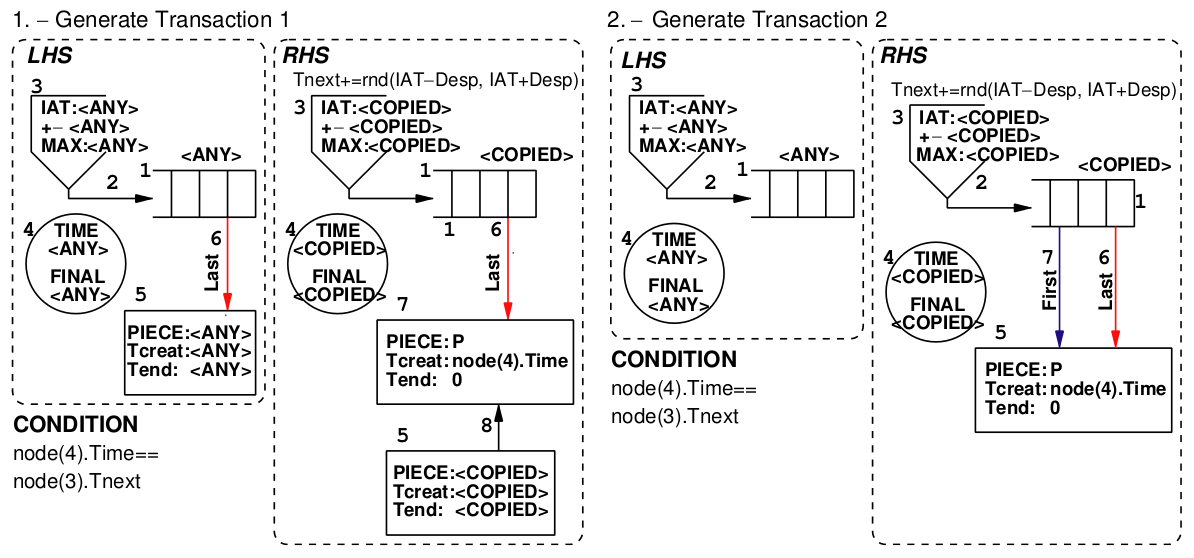
\includegraphics[width=0.9\textwidth]{1.png}
    \caption{Фрагмент семантики симуляции для дискретно-событийной модели (рисунок взят из работы~\cite{atom3})}
    \label{fig1}
  \end{center}
\end{figure}

Формально, на рис.~\ref{fig1} изображён фрагмент семантики симуляции для описанной выше дискретно-событийной модели. На нём присутствуют основные два из шести правил данной семантики. Они оба разбирают случай создания новой задачи генератором и могут быть применены только тогда, когда системное время совпадает с временем, когда новая задача должна быть сгенерирована. Об этом говорит условие (CONDITION) в левой части каждого из правил. node(4) является синтаксическим способом получить доступ к узлу с меткой 4, т.е. к таймеру, атрибут Time которого и есть системное время. Атрибут Tnext узла с меткой 3, т.е. генератора, является временем генерации новой задачи.

Правило 1, имеющее имя “Generate Transaction 1”, осуществляет генерацию новой задачи в тот момент, когда очередь задач не пуста. Правило 2 с именем “Generate Transaction 2” устроено аналогично и рассматриваться не будет. Оно разбирает случай, когда очередь пуста. Остановимся подробнее на правиле 1.

Элемент с меткой 1 является очередью, 2 --- связь между генератором и соответствующей ему очередью, 3 --- сам генератор, 4 ---таймер, 5 --- задача, 6 --- связь с меткой Last, указывающая на последний элемент в очереди, 7 --- новай сгенерированная задача, 8 --- обычная связь между задачами в списке задач очереди.

Существование связи с меткой Last говорит о том, что очередь в данном случае не пуста. Раз в левой части правила напротив всех атрибутов различных элементов стоит метка “ANY”, то никаких дополнительных условий на их значение не накладывается. В правой части видно создание новой задачи (узел с меткой 7), добавление связи с меткой 8 и изменение конца связи с меткой 6. Наличие такого числового соответствия элементов позволяет быстро понимать, что изменилось в графе, без всякой дополнительной информации. В итоге получаем, что новая задача добавилась в конец списка задач очереди.

При создании новой задачи её атрибутам были заданы некоторые как фиксированные значения, так и основанные на значениях других элементов. Например, времени создания (Tcreat) было присвоено значение текущего системного времени (node(4).Time). Также можно присваивать значения и другим атрибутам. К атрибуту генератора Tnext, означающего время генерации новой задачи, было добавлено некоторое выражение, основанное на значениях его же атрибутов. Остальные же значение атрибутов элементов были просто скопированы при помощи метки “COPIED”.

С организацией преобразования дискретно-событийной модели к сетям Петри, их оптимизацией и генерацией кода в GPSS можно ознакомиться подробнее в самой статье~\cite{atom3}. Для трансформации в сети Петри активно используется обобщённая связь, упомянутая ранее, а для оптимизации и генерации кода используется набор действий, исполняемых после применения правила.

\subsection{Анализ}

Подход к заданию семантики интерпретации, использованный в проекте AToM$^3$, фактически является частичной реализацией формального DMM-подхода с расширением в виде возможности ставить дополнительные условия на значения атрибутов элементов для применения правил, а также производить некоторый набор операций после непосредственного изменения модели. В связи с этим на него распространяется то же замечание про NP-полноту задачи поиска подграфа, что и на DMM-подход. Возможность конвертации моделей на одном языке в другой, а также изменение модели в оптимизационных целях являются отличительными составляющими данного подхода.

Формально подход, реализованный в AToM$^3$, в сравнении с xUML и EProvide почти полностью совпадает с DMM-подходом. Существенным улучшением DMM-подхода является возможность задавать ограничения на применение правил при помощи OCL или на языке Python и исполнять определённый код на языке Python после применения правила. Причём оба этих механизма имеют полный доступ ко всем элементам, содержащимся в правиле. Благодаря этому данный подход становится больше похож на реализацию подхода из EProvide с использованием графической нотации задания преобразований моделей.

Также данный подход от DMM отличает некомпактный способ задания правил преобразования. Нужно явно указывать левую и правую часть и задавать соответствие элементов индексами. Зато для атрибутов в левой части можно указывать значение “ANY”, когда не важно, чему он равен, в правой части --- “COPIED”, если при применении правила значение нужно скопировать, и в обоих частях --- “SPECIFIED”, если значение задаётся явно.

\section{Анимированная симуляция диаграмм на базе GenGED}

Описание данного подхода изложено в статьях~\cite{genged1, genged2, genged3} на различных примерах. В~\cite{genged3} рассматривается система, состоящая из набора ресторанов, обслуживающих очереди покупателей на машинах. В~\cite{genged1} приводится пример анимации работы лифта при помощи сетей Петри, а в~\cite{genged2} разобрана проблема обедающих философов. Главным в этом подходе является тот факт, что при интерпретации пользователь видит не изменение диаграммы на визуальном языке, а некоторую анимацию.

\subsection{Описание подхода}

Представление предметной области задачи и самой задачи в виде визуального языка моделирования и с его помощью созданной диаграммы, соответственно, и последующая интерпретация диаграммы в терминах этого же визуального языка порой являются недостаточно очевидными для пользователей, не являющихся разработчиками этого языка. Переход от диаграмм к реальным анимационным картинкам, которые будут непрерывно изменяться при интерпретации, как видеофильм, должен сгладить этот семантический разрыв.

Как показано на рис.~\ref{fig2}, основой для всего процесса анимации является некоторая поведенческая модель (UML behavioral model), записанная при помощи UML. Для исполнения она переводится в симуляционную систему (simulation system), на экран же пользователю выводится набор анимационных представлений (animation views). В симуляционной системе модель переходит из состояния в состояние при помощи симуляционных шагов (simulation steps), а в анимационных представлениях используются анимационные шаги (animation steps).

\begin{figure} [ht]
  \begin{center}
    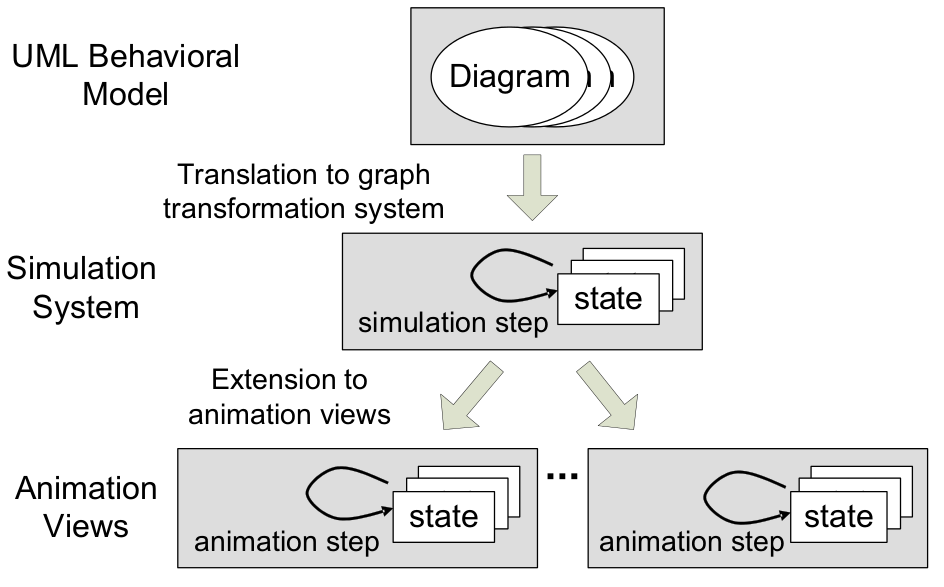
\includegraphics[width=0.9\textwidth]{2.png}
    \caption{Формальная схема анимационного представления исполнения (этот и все последующие в этом разделе рисунки взяты из работы~\cite{genged3})}
    \label{fig2}
  \end{center}
\end{figure}

Система, заданная при помощи набора UML диаграмм, представляется в виде объектной UML диаграммы, формализованной как граф, а сам процесс исполнения заключается в преобразовании этой диаграммы. Для того чтобы работать с анимационным представлением, не выходя за рамки объектных диаграмм, производится расширение набора способов визуализации вершин графа модели путём добавление новых классов в диаграмму классов, описывающую предметную область. Подробнее об этом расширении будет рассказано в следующем разделе на конкретном примере.

В рамках способа задания семантики в данном подходе используются правила преобразования графов с ограничениями на языке OCL как на уровне симуляции, так и на уровне анимации. Для обеспечения анимации сценариев предлагается использовать средство GenGED\footnote{GenGED, URL: \url{http://user.cs.tu-berlin.de/~genged}. Дата обращения: 01.03.2013}, позволяющее расширять системы преобразования графов такой функциональностью и экспортировать результат в формат SVG\footnote{Scalable Vector Graphics, \url{http://www.w3.org/TR/svg}. Дата обращения: 01.03.2013}. Рассмотрим данный подход более подробно на примере систем ресторанов и покупателей.

\subsection{Пример анимации системы ресторанов}

Рассматриваемая система состоит из набора ресторанов, обеспечивающих обслуживание потребителей на автомобилях. У ресторанов могут возникать очереди, в таком случае они обрабатываются последовательно. Потребители могут находится в состоянии простоя, ожидания оплаты и в состоянии, когда они уже оплатили заказ и готовы его съесть.

Вначале вся система описывается при помощи набора UML-диаграмм. Так, диаграмма классов используется для общего описания объектов предметной области и их взаимоотношений, диаграммы кооперации для определения возможного поведения объектов и протокольные диаграммы состояний, следящие за правильным порядком использования определённых операций. Диаграмма кооперации раскрывает значение операций, объявленных в диаграмме классов. рис.~\ref{fig3a} и рис.~\ref{fig3b} демонстрирует пару таких диаграмм.

На рис.~\ref{fig3a} изображена общая диаграмма классов для рассматриваемой системы. Она состоит из четырёх классов: клиент (Client), заказ (Order), еда (Meal) и магазин (DriveThrough). Клиент может посещать магазин (отношение Visit), делать заказ (отношение Submit) и получать свою еду (отношение ToEat). Магазин же может готовить еду (отношение ToServe). Клиент встаёт в очередь и делает заказ при помощи метода queueAndOrder(), платит за него и ест при помощи методов pay() и eat(). Также он может обработать событие ready(meal:Meal), сообщающее, что еда meal готова. Основные методы, например, обслужить (serve()), для магазина показаны в соответствующем блоке.

\begin{figure} [ht]
  \begin{center}
    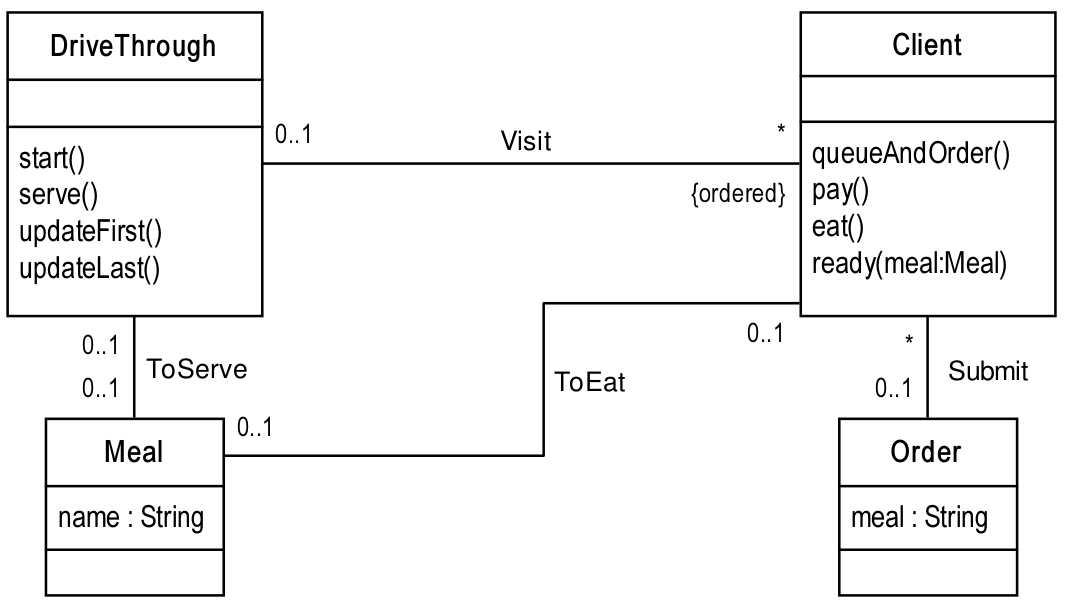
\includegraphics[width=0.9\textwidth]{3a.png}
    \caption{Диаграмма классов для системы ресторанов}
    \label{fig3a}
  \end{center}
\end{figure}

\begin{figure} [ht]
  \begin{center}
    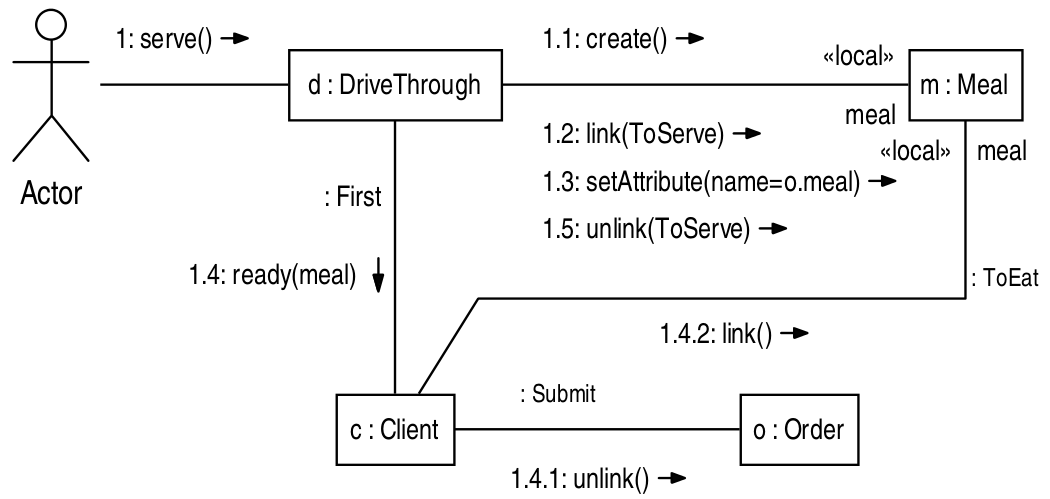
\includegraphics[width=0.9\textwidth]{3b.png}
    \caption{Диграмма кооперации для операции serve()}
    \label{fig3b}
  \end{center}
\end{figure}

Пример диаграмма кооперации для операции serve() показан на рис.~\ref{fig3b}. Она работает по следующему принципу. Клиент инициирует в магазине выполнение метода serve() с номером 1. При его исполнении сначала создаётся объект класса Meal (действие 1.1) и задается, что он должен быть обработан рестораном (действие 1.2). Затем атрибуту объекта класса Meal присваивается соответствующее значение из объекта заказа (действие 1.3). Ресторан посылает потребителю сообщение о том, что еда готова (действие 1.4), заказ открепляется от потребителя (действие 1.4.1), и появляется связь между потребителем и едой, означающая, что потребитель готов данную еду употребить (действие 1.4.2). Потом еда отцепляется от магазина (действие 1.5).

После этого на основе диаграмм коопераций и используемых в них операций составляется набор правил преобразования графов, соответствующих им. На рис.~\ref{fig3b} такими являются, например, create(), link(), unlink() и т.п. рис.~\ref{fig4} показывает правило для операции create(). Как видно из рисунка, левая часть правила состоит из магазина d, первого в очереди клиента c, о чём говорит связь типа First между ним и магазином, который сделал заказ o на еду x, о чём говорит связь типа Submit. В правой же части этого правила добавлен элемент m типа Meal с названием еды, совпадающим с названием еды в заказе, т.е. x. Таким образом, правило просто добавляет элемент с нужным видом еды в модель.

\begin{figure} [ht]
  \begin{center}
    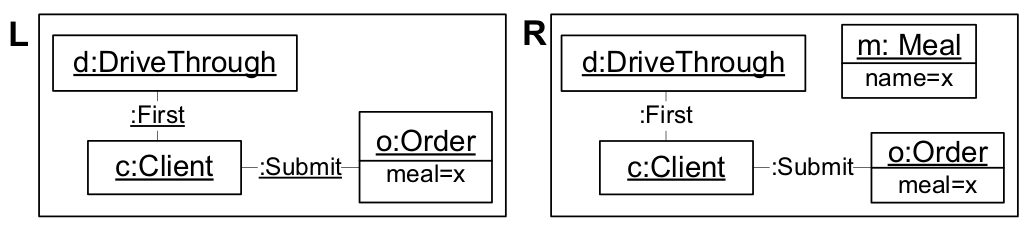
\includegraphics[width=0.9\textwidth]{4.png}
    \caption{Правило преобразования графов для операции create() с рис.~\ref{fig3b}}
    \label{fig4}
  \end{center}
\end{figure}

Для отображения текущего состояния системы в данном подходе используются объектные диаграммы, как было отмечено в параграфе 4.1. В связи с этим правила преобразования графов задаются именно для них, как видно из рис.~\ref{fig4}. Для того, чтобы перейти от объектных диаграмм к анимационному представлению, вначале нужно расширить систему отображения элементов графов таких диграмм.

Расширение изображено на рис.~\ref{fig5} и может также содержать дополнительную информацию об ограничениях по расположению этих элементов. Например, автомобиль всегда должен находиться на дороге и т.п. Из рисунка видно, что мы добавили класс Building для отрисовки здания магазина, класс Car, соответствующий клиенту, класс OrderBubble соответствует заказу, а класс ServedMeal --- еде. Атрибуты этих классов дублируют атрибуты соответствующих им классов. Это расширение в данном примере выглядит бессмысленно в силу фактического повторения описания классов исходной системы, но в других случаях, например, анимации работы лифта~\cite{genged1}, основанной на сетях Петри, данные наборы классов отличаются коренным образом.

Поскольку подход основан на представлении системы в виде набора UML диаграмм, то данное расширение подразумевает лишь создание новых классов в исходной диаграмме классов, определение способов отображения объектов данных классов и ограничения на их расположение. Вся работа с графикой в дальнейшем осуществляется при помощи GenGED.

\begin{figure} [ht]
  \begin{center}
    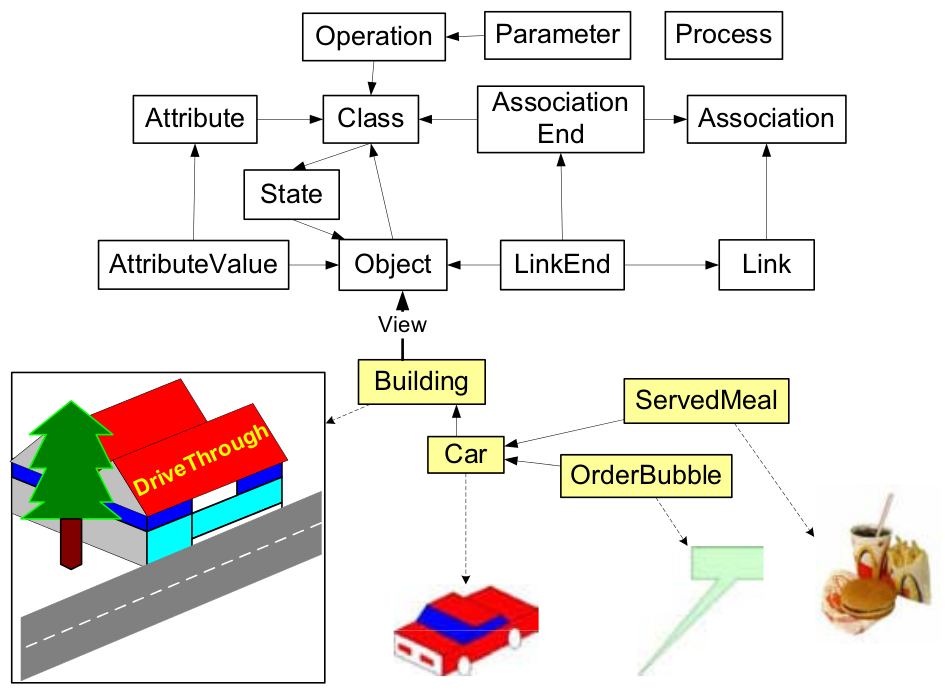
\includegraphics[width=0.9\textwidth]{5.png}
    \caption{Расширение типизированного графа для системы ресторанов}
    \label{fig5}
  \end{center}
\end{figure}

После такого расширения необходимо изменить уже существующие правила преобразования графов с учётом добавленных объектов, а также добавить несколько новых, специфичных для анимированного отображения.

На рис.~\ref{fig6a} и рис.~\ref{fig6b} показана часть этих новых правил, при помощи которых при интерпретации будет изменяться анимационное представление. Буква “N” у правой части каждого правила означает, что для правила существуют отрицающее применение условие (NAC, подробнее о том, что это такое --- в статье~\cite{part1}), совпадающее со всем изображённым в правой части графом. Таким образом, каждое правило может быть применено ровно один раз для каждого потребителя (и инициализация системы тоже случится ровно один раз). Также можно заметить, что все эти правила изменяют только анимационное представление (цветные элементы) и никак не трогают исходную объектную модель (белые элементы), а значит они никак не зависят от существующих правил, таких как на рис.~\ref{fig4}.

Например, правило initDriveThrough, изображённое на рис.~\ref{fig6a}, по своему смыслу рисует на экране ресторан, а в рамках объектной модели присоединяет объект класса Building к соответствующему объекту магазина. Для применения правила необходимо лишь существование в системе, т.е. в исходной объектной модели, магазина.

\begin{figure} [ht]
  \begin{center}
    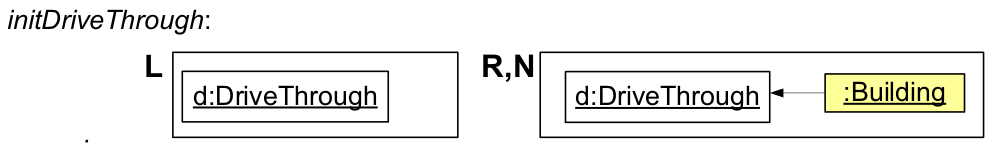
\includegraphics[width=0.9\textwidth]{6a.png}
    \caption{Правило инициализации магазина}
    \label{fig6a}
  \end{center}
\end{figure}

Правило ordering, представленное на рис.~\ref{fig6b}, предназначено для анимации осуществления клиентом заказа в магазине. В результате на экране над соответствующей машиной появится информационное сообщение с текстом заказа. В объектную модель добавляется экземпляр OrderBubble со значением атрибута названия еды, совпадающим со значением атрибута meal заказа o. Для применения правила необходимо, чтобы клиент уже сделал заказ на уровне исходной объетной модели.

\begin{figure} [ht]
  \begin{center}
    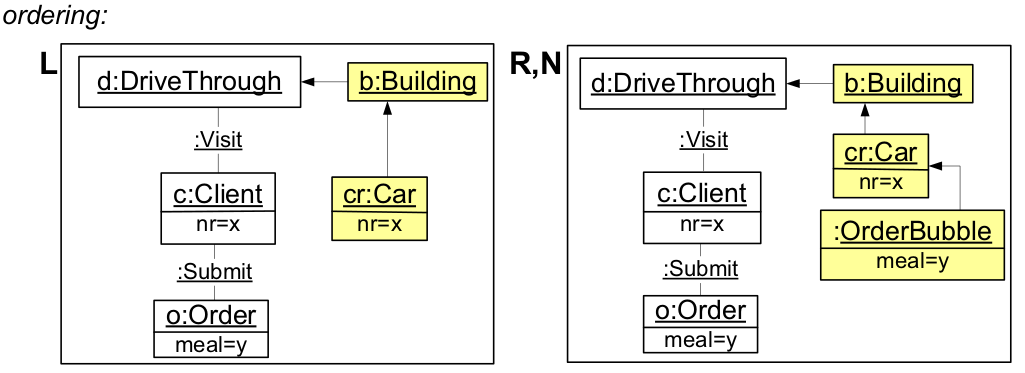
\includegraphics[width=0.9\textwidth]{6b.png}
    \caption{Правило осуществления клиентом заказа}
    \label{fig6b}
  \end{center}
\end{figure}

В качестве примера изменённого специально для анимационного представления правила рассмотрим правило ready(). Как видно из рис.~\ref{fig7}, оно целиком содержит правило преобразования графов для обычной симуляции (белые элементы), т.е. отсоединение заказа o от клиента и присоединение к нему еды m. В обычной объектной модели эти операции бы означали, что еда для клиента была приготовлена и доставлена ему. При анимации же необходимо заменить рисунок с заказом на пиктограмму приготовленной еды, что и происходит, исходя из изменений графа, состоящего из цветных элементов (исчез экземпляр OrderBubble и добавился экземпляр ServedMeal). Важно отметить, что в данном подходе никакие элементы начального графа не удаляются. Например, OrderBubble не исчезнет из модели, а при помощи GenGED станет невидимым.

\begin{figure} [ht]
  \begin{center}
    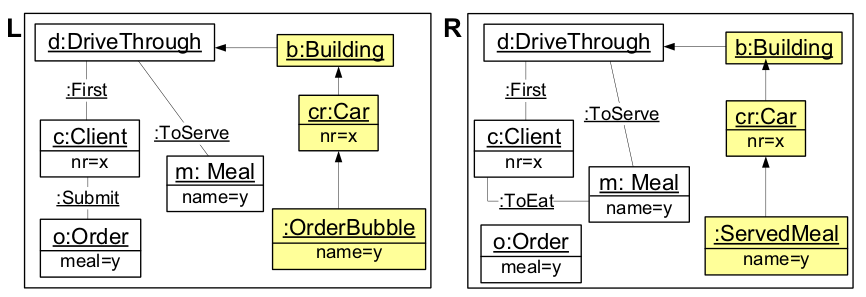
\includegraphics[width=0.9\textwidth]{7.png}
    \caption{Правило ready() для анимационного представления}
    \label{fig7}
  \end{center}
\end{figure}

Процесс непосредственной симуляции анимационного представления представлен на рис.~\ref{fig8}. В магазин приехали два клиента и организовали очередь. Первый при помощи правила order() сделал заказ на еду с названием “Meal 1”, появляется соответствующий диалоговый пузырь. Магазин обслуживает данный заказ при помощи правила serve(), и напротив клиента появляет пиктограммка еды. Затем клиент ест еду при помощи правила eat(), что удаляет пиктограммку еды и выводит его из очереди. Непрерывность движения машин достигается при помощи GenGED определением операции линейного движения перед постановкой машины в очередь, а также после употребления еды потребителем.

\begin{figure} [ht]
  \begin{center}
    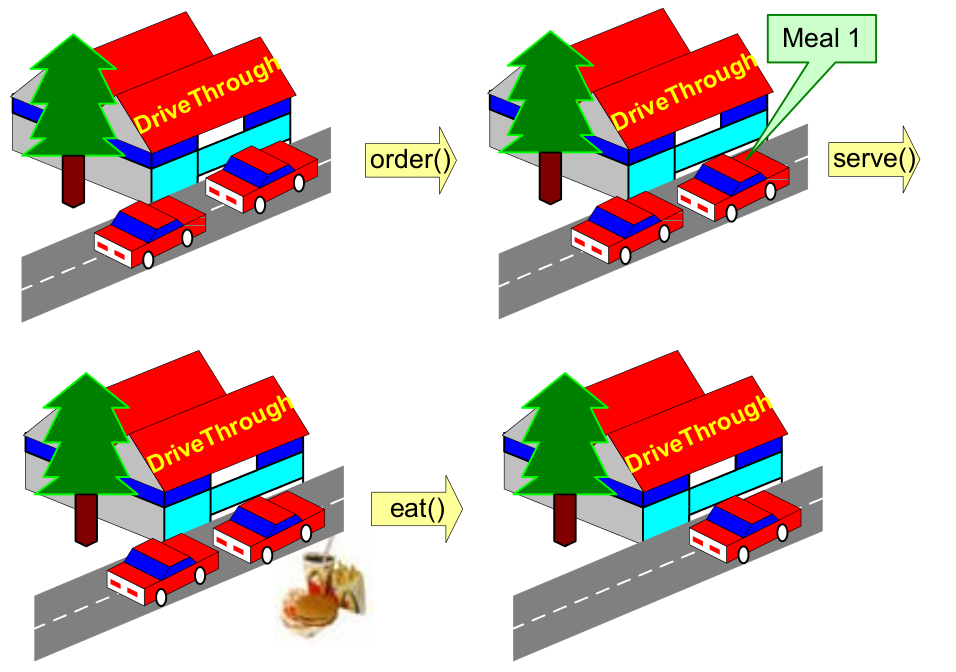
\includegraphics[width=0.9\textwidth]{8.png}
    \caption{Симуляция системы}
    \label{fig8}
  \end{center}
\end{figure}

\subsection{Анализ}

В плане способа задания семантики данный подход полностью основывается на технологии преобразования графов, что даёт возможность создавать наглядные и понятные операционные семантики. С их помощью данный подход позволяет задавать реальное исполнение различных поведенческих UML-диаграмм (например, диаграмм кооперации и протокольных диаграмм состояний), при помощи которых описывается разрабатываемая система. Также показано её применение для создания нового уровня представления интерпретации системы в виде анимации. Использование данного подхода при задании семантики исполнения позволяет существенно сократить разрыв между предметной областью и её представлением в системе.

Как и все остальные подходы, использующие преобразования графов, из-за NP-полноты задачи поиска подграфа в графе, на больших графах возможно значительное уменьшение производительности, в отличие от подходов, использованных в xUML или в EProvide.

По фактическому содержанию данный подход является некоторым упрощением способа, использующегося в AToM$^3$, т.к. не позволяет задавать на языке Python дополнительные ограничения на применение правил и исполнять некоторый код после применения. Таким образом, сравнение его с остальными подходами аналогично уже приведённым сравнениям. Однако главным недостатком, в отличие от DMM или AToM$^3$, является его неуниверсальность, а именно тот факт, что исходную систему нужно описывать набором UML диаграмм и что исполняемая модель будет представлять собой объектную диаграмму. Существенным плюсом же является то, что процесс визуализации интерпретации происходит максимально понятно для пользователя, т.к. используются не простые диаграммы, а анимация.

\section{Сравнительный анализ разобранных подходов}

Основные сходства и различия описанных способов задания семантики интерпретации визуальных языков можно увидеть в табл. 1. Сравнение подходов осуществлялось по шкале от 0 до 3 по следующим критериям.

Универсальность --- это возможность задания семантики для произвольных визуальных языков, т.е. оценка того, насколько подход подходит под концепцию метамоделирования. Двухуровневая отладка совсем не соответствует концепции метамоделирования и DSM, т.к. данный подход ориентирован на создание единичного отладчика для определённого языка и не подразумевает удобного обобщения (0 баллов), UML и анимационный подход работают так или иначе только с диаграммами UML (0 баллов), в то время как остальные способы не зависят от входного визуального языка (3 балла).

Задание семантики на основе хорошо определённого (математически) подхода добавляет программам доказуемость и предсказуемость поведения, т.е. при таком задании невозможна различная интерпретация спецификации, которая бы присутствовала, например, в большом текстовом описании. За это отвечает критерий формальности. DMM, AToM$^3$ и анимационный подходы основаны на технологии преобразования графов (3 балла), EProvide поддерживает задание семантики, основанной на стандарте QVT Relation, а xUML базируется на PAS, которая была стандартизирована Object Management Group в 2001 году (1 балл, так как основаны на стандартах).
  
Наглядность средств задания семантики определяется тем, визуально (3 балла) ли это нужно делать или при помощи текста (0 баллов). Подходы, основанные на преобразованиях графов, т.е. DMM, AToM$^3$ и анимационный, являются большей частью визуальными, а остальные --- текстовыми. xUML, благодаря своей визуальной составляющей в виде диаграмм состояний жизненных циклов объектов, мы оцениваем в 1 балл.

Наглядность процесса интерпретации зависит от того, как эта интерпретация будет отображаться пользователю. Самым наглядным из рассмотренных подходов является анимационный подход, т.к. там пользователю представляются реальные картинки, объединённые в анимацию (3 балла). DMM, EProvide и AToM$^3$ будут по ходу исполнения изменять модель, а также при необходимости подсвечивать отдельные элементы, как, например, в EProvide, поэтому по этому критерию мы оцениваем их все в 2 балла. При использовании xUML или двухуровневой отладки интерпретация позволит лишь подсвечивать текущий исполняемый элемент (1 балл).

Если смотреть на способы задания семантики со стороны разработчика конкретного визуального языка, то важным критерием их сравнения становится понятность, отвечающая за количество знаний в области визуального моделирования и других связанных с ней областях, которое необходимо иметь для успешного и осмысленного применения данных способов. На наш взгляд, самым понятным подходом является DMM, т.к. правила преобразования графов воспринимаются интуитивно. У AToM$^3$ и анимационного подхода есть недостаток в том, что возможно ставить различные ограничения и писать исполняемые инструкции на OCL и Python,  а это требует от разработчика дополнительных знаний. Для анимационного подхода также нужно частичное знание UML, поэтому мы оцениваем его в 1 балл, а AToM$^3$ --- в 2 балла. xUML подразумевает сложную систему зависимостей диаграмм друг от друга, а также активную работу с AL, что снижает понятность, т.к. необходимо хорошо ориентироваться в UML и в PAS или некотором AL (0 баллов). Для использования EProvide нужно изучить стандарт QVT Relation, что по сложности сравнимо с подходом в xUML (0 баллов). Для применения двухуровневой отладки же необходимо знание языка программирования, на котором написана использующаяся система, а также особенностей её реализации для того, чтобы было возможно встраивание в неё функционала отладчиков, что даёт данному подходу оценку в 0 баллов.

Критерий наличия реализации в комментариях не требуется (для xUML их существует много). 3 балла, если реализация существует, 0 баллов, если нет. Двухуровневая отладка имеет 1 балл, т.к. для неё присутствует реализация для конкретного языка. Если для данного подхода уже реализовано средство, позволяющее не только интерпретировать, но и отлаживать, т.е. использовать различные точки останова, просмотр и изменение значений атрибутов и т.п., или для подхода возможно такое расширение, то он имеет 3 балла в графе “возможность создания отладчика”, иначе --- 0 баллов. Как видно из обзора, анимационный подход не подразумевает отладки напрямую, т.к. пользователь видит лишь анимацию интерпретации.

\begin{table}[h]
\begin{center}
\begin{tabular}{| p{0.2\linewidth} | p{0.1\linewidth} | c|c|c|c|c|}
  \hline
  Критерий сравнения                              & Двухур. отладка & xUML & DMM & EProvide & AToM$^3$ & Ани\-ма\-ция \\   \hline  
  Универ\-саль\-ность                             & 0               & 0    & 3   & 3        & 3     & 0        \\   \hline  
  Фор\-маль\-ность                                & 0               & 1    & 3   & 1        & 3     & 3        \\   \hline  
  Наглядность средств \par задания \par семантики & 0               & 1    & 3   & 0        & 3     & 3        \\   \hline  
  Наглядность процесса интерпретации              & 1               & 1    & 2   & 2        & 2     & 3        \\   \hline  
  Понятность                                      & 0               & 0    & 3   & 0        & 2     & 1        \\   \hline  
  Наличие реализации                              & 1               & 3    & 0   & 3        & 3     & 3        \\   \hline  
  Возможность создания отладчика                  & 3               & 3    & 3   & 3        & 3     & 0        \\   \hline  
\end{tabular}
\end{center}
\caption{ Сравнительная таблица для разобранных подходов}
\label{table1}
\end{table}


После суммирования полученных для каждого из подходов баллов получается следующее распределение: двухуровневая отладка --- 5 баллов, xUML --- 9 баллов, EProvide --- 12 баллов, анимационный подход --- 13 баллов, DMM --- 17 баллов, AToM$^3$ --- 19 баллов. Благодаря наличию реализации, подход, использующийся в AToM$^3$, мы считаем лучшим подходом. Он очень похож на DMM, что подтверждают набранные ими баллы.

\section{Дискуссия и заключение}

Переход от текстового программирования к программированию графическому в случае языков общего назначения не всегда приводит к существенному повышению производительности труда конечных разработчиков, поскольку неявно подразумевает создание громоздких моделей, сложных для восприятия и модификации. Бороться с этим можно использованием специализированных языков, каждый из которых обычно создается для решения лишь определенного круга задач. Как правило, такие языки гораздо более наглядны (элементы языка напрямую представляют сущности предметной области, понятные даже людям, не обладающим навыками программирования) и хорошо подходят для автоматической кодогенерации по моделям, составленным с их помощью (в силу ограниченности предметной области). 

Существенную роль в предметно-ориентированном моделировании играют DSM-платформы --- окружения, позволяющие автоматизированно создавать инструментальную поддержку для разрабатываемых DSL по формальным описаниям определенных аспектов этих языков (например, по описанию абстрактного и конкретного синтаксиса языка возможна автоматическая генерация полноценного визуального редактора для работы с этим языком). Для поведенческих языков огромную роль играет их семантика --- значение как элементов языка по отдельности, так и конструкций, из них составляемых. Имея должное формальное описание семантики, DSM-платформа может позволить автоматически сгенерировать интерпретатор или отладчик для данного языка, расширяя набор инструментальных средств DSM-решения и облегчая работу его пользователей.

Для формального описания операционной семантики графических языков, на наш взгляд, очень хорошо подходят графовые грамматики и механизмы преобразования графов с их помощью. Задавая правила преобразований, разработчик DSM-решения оперирует не в терминах абстрактных сущностей, а напрямую элементами создаваемого языка, наглядно визуализируя происходящие с моделями в процессе исполнения действия. Несмотря на то, что разработчик (или группа разработчиков) DSM-решения должен обладать квалификацией гораздо более существенной, нежели будущие пользователи данного DSM-решения, удобство и наглядность используемых ими инструментов DSM-платформы также имеет большое значение: чем быстрее DSM-решение будет готово, тем быстрее оно поступит к своим пользователям; чем меньше будут ошибаться разработчики DSM-решения, тем более качественной и точной получится финальная среда разработки, тем выше будет степень удовлетворенности и продуктивность работы ее пользователей --- тем быстрее компания будет получать пользу от внедрения DSM-подхода. В этом свете подходы, основанные на графовых грамматиках и преобразовании графов, видятся нам довольно удачным способом задания семантики исполнения визуальных языков --- формальным, компактным, наглядным.

На основе анализа рассмотренных в статье методов можно предложить следующий подход, сочетающий в себе их лучшие стороны. В качестве графической составляющей задания семантики можно использовать технологию преобразования графов, описанную в DMM. Дополнительные ограничения на применение правил для компактности можно записывать при помощи текстового языка (например, с помощью широко распространенного языка задания ограничений OCL). Для класса языков, формализуемых с помощью сетей Петри, визуализацию потока исполнения можно реализовать, введя в язык описания семантики специальный маркер. Связь произвольного элемента языка с данным маркером будет указывать на элемент модели, исполняемый в текущий момент (при желании визуализировать процесс исполнения этот элемент может быть подсвечен или как-то иначе выделен относительно остальных). 

При необходимости выполнять какие-то нетривиальные действия при выполнении определенного правила (например, менять значения свойств элементов), можно ввести понятие реакции на применение правила --- ассоциировать с каждым правилом код на некотором интерпретируемом языке (например, на Python, как в AToM$^3$), который будет исполняться при исполнении данного правила. Подобный механизм можно распространить и на отдельные элементы --- задавать код, исполняемый при прохождении потока исполнения через узел данного типа. В частности, это позволит использовать данный подход и для создания генераторов кода по моделям --- при прохождении интерпретатора через элементы модели будут генерироваться соответствующие им артефакты (например, части документации или исходного кода). Разумеется, для создания генераторов для языков со сложным потоком исполнения может потребоваться нетривиальный анализ моделей (например, поиск циклов), что приведет к существенному усложнению кода реакций на правила. Однако, так как в рамках предметно-ориентированной парадигмы приоритет обычно отдается небольшим и несложным логически языкам, такой подход может быть вполне достаточен для довольно широкого круга задач.


\begin{thebibliography}{9001}
\bibitem{kartashev} \emph{Карташев М.} Двухуровневая схема отладки // Системное программирование. Под ред. А. Н. Терехова, Д. Ю. Булычева. Изд-во СПбГУ, 2004. С. 348-365.
\bibitem{koznov1} \emph{Кознов Д.В.} Разработка и сопровождение DSM-решений на основе MSF // Системное программирование. Под ред. А. Н. Терехова, Д. Ю. Булычева. Изд-во СПбГУ, 2008. Т. 3. № 1. С. 80-96.
\bibitem{koznov2} \emph{Павлинов А., Кознов Д., Перегудов А. и др.} О средствах разработки проблемно-ориентированных визуальных языков // Системное программирование / Вып. 2, под ред. А. Н. Терехова и Д. Ю. Булычева. СПб.: Изд. СПбГУ, 2006. С. 116-141.
\bibitem{part1} \emph{Поляков В., Брыксин Т.} Подходы к заданию семантики интерпретации диаграмм в рамках DSM-подхода // Системное программирование / Вып. 7, под ред. А. Н. Терехова и Д. Ю. Булычева. СПб.: Изд. СПбГУ, 2012, С. 156-183 
\bibitem{koznov3} \emph{Сорокин А., Кознов Д.} Обзор Eclipse Modeling Project // Системное программирование / Вып. 5, под ред. А. Н. Терехова и Д. Ю. Булычева. СПб.: Изд. СПбГУ, 2010. С. 6-31.
\bibitem{genged1} \emph{Ehrig H., Ermel C., Taentzer G.} Simulation and Animation of Visual Models of Embedded Systems // Embedded Systems – Modeling, Technology, and Applications, Springer, 2006, P. 11-20.
\bibitem{genged2} \emph{Ermel C., Ehrig K.} View Transformation in Visual Environments applied to Algebraic High-Level Nets // Electronic Notes in Theoretical Computer Science, Vol. 127, Issue 2, 2005, P. 61–86.
\bibitem{genged3} \emph{Ermel C., Holscher K., Kuske S., Ziemann P.} Animated Simulation of Integrated UML Behavioral Models based on Graph Transformation // IEEE Symposium on Visual Languages and Human-Centric Computing (VL/HCC'05), 2005, P. 125-133.
\bibitem{atom1} \emph{Fishman G.} Discrete event simulation, Modeling, Programming and Analysis // Springer Series in Operations Research, Springer, New York, 2001. 537 p.
\bibitem{gpss} \emph{Gordon G.} System Simulation // 2nd Edition, Prentice-Hall, Englewood Cliffs, NJ, 1996. 303 p.
\bibitem{dmm1} \emph{Hausmann J.} Dynamic Meta Modeling: A Semantics Description Technique for Visual Modeling Languages. PhD Thesis, 2005, Paderborn, Faculty of Computer Science, Electrical Engineering, and Mathematics of the University of Paderborn. 326 p.
\bibitem{sem2} \emph{Kahn G.} Natural Semantics // Proceedings of the 4th Annual Symposium on Theoretical Aspects of Computer Science, Springer-Verlag, London, 1987, P. 22-39.
\bibitem{sem1} \emph{Hoare C. A. R.} An axiomatic basis for computer programming // Communications of the ACM, 12(10):576–580, 1969, P. 576-583.
\bibitem{dsmbook} \emph{Kelly S., Tolvanen J.} Domain-Specific Modeling: Enabling Full Code Generation // Wiley-IEEE Computer Society Press, 2008. 448 p.
\bibitem{atom2} \emph{Lara J., Vangheluwe H.} AToM$^3$ : a tool for multi-formalism modelling and meta-modelling // Proceedings of ETAPS/FASE’02, Lecture Notes in Computer Science, Vol. 2306, Springer, Berlin, 2002, P. 174–188.
\bibitem{atom3} \emph{Lara J., Vangheluwe H.} Defining visual notations and their manipulation through meta-modelling and graph transformation // Journal of Visual Languages and Computing 15, 2004, P. 309–330.
\bibitem{xuml} \emph{Mellor S., Balcer M.} Executable UML: A foundation for model-driven architecture // Addison Wesley, 2002. 416 p.
\bibitem{uml} \emph{} OMG Unified Modeling Language, Superstructure. Version 2.4.1. OMG. 2011. 732 p.
\bibitem{sem3} \emph{Plotkin G.} A Structural Approach to Operational Semantics // Technical Report DAIMI FN-19, University of Aarhus, 1981. 133 p.
\bibitem{eprov1} \emph{Sadilek D., Wachsmuth G.} Prototyping Visual Interpreters and Debuggers for Domain-Specific Modelling Languages // ECMDA-FA 2008, LNCS 5095, 2008, P. 64–79.
\bibitem{sem3} \emph{Scott D., Strachey C.} Towards a Mathematical Semantics for Computer Languages // Computers and Automata, Wiley, 1971, P. 19–46.
\bibitem{sem4} \emph{Slonneger K., Kurtz B.} Syntax and Semantics of Programming Languages, A Laboratory Based Approach // Addison-Wesley Publishing, 1995. P.187-222.
\bibitem{eprov2} \emph{Wachsmuth G.} Modelling the Operational Semantics of Domain-Specific Modelling Languages // Generative and Transformational Techniques in Software Engineering II. Lecture Notes in Computer Science Volume 5235, Springer, 2008, P. 506-520.
\bibitem{ocl} \emph{Warmer J., Kleppe A.} The Object Constraint Language: Precise Modeling with UML // Addison- Wesley Object Technology Services, Reading, MA, 1999. 144 p.
\bibitem{dsm1} \emph{Isazadeh H.} Architectural Analysis of MetaCASE. A Study of Capabilities and Advances. Thesis for the degree of Master of Science. URL: www.collectionscanada.gc.ca/obj/s4/f2/dsk2/ftp04/mq20654.pdf. Дата обращения: 01.03.2013 
\bibitem{graph} \emph{Rozenberg G.} Handbook of Graph Grammars and Computing by Graph Transformation. Volume 1: Foundations. World Scientific, 1997.
\bibitem{dsm2} \emph{Jézéquel J.-M., Barais O., Fleurey F.} Model Driven Language Engineering with Kermeta. Generative and Transformational Techniques in Software Engineering III, Lecture Notes in Computer Science, Volume 6491, 2011, p. 201-221
\bibitem{dsm3} \emph{Bardohl R., Ermel C., Weinhold I.} GenGED – A Visual Definition Tool for Visual Modeling Environments. Applications of Graph Transformations with Industrial Relevance, Lecture Notes in Computer Science, Volume 3062, 2004, p. 413-419
\bibitem{dsm4} \emph{Amyot D., Farah H., Roy J.-F.} Evaluation of Development Tools for Domain-Specific Modeling Languages, 5th International Workshop, SAM 2006, Kaiserslautern, Germany, May 31 - June 2, 2006, Springer Berlin Heidelberg, pp. 183-197
\end{thebibliography}

\end{document}
